%% LyX 2.1.3 created this file.  For more info, see http://www.lyx.org/.
%% Do not edit unless you really know what you are doing.
\documentclass[12pt,english,hidelinks]{article}
\renewcommand{\familydefault}{\rmdefault}
\usepackage[utf8x]{inputenc}
\usepackage{geometry}
\geometry{verbose,tmargin=2cm,bmargin=2cm,lmargin=3cm,rmargin=2cm}
\usepackage{babel}
\usepackage{array}
\usepackage{calc}
\usepackage{textcomp}
\usepackage{graphicx}
\usepackage{setspace}
\PassOptionsToPackage{normalem}{ulem}
\usepackage{ulem}
\usepackage{subscript}
\onehalfspacing
\usepackage{amssymb}
\usepackage{amsmath}
\usepackage{enumerate}
\usepackage[unicode=true]
 {hyperref}

\makeatletter

%%%%%%%%%%%%%%%%%%%%%%%%%%%%%% LyX specific LaTeX commands.
%% Because html converters don't know tabularnewline
\providecommand{\tabularnewline}{\\}

%%%%%%%%%%%%%%%%%%%%%%%%%%%%%% User specified LaTeX commands.
\usepackage{fixltx2e}

\makeatother

\begin{document}
\pagestyle{empty}

\begin{center}
UNIVERSITATEA ALEXANDRU IOAN CUZA IAŞI
\par\end{center}

\begin{center}
\textbf{\large{}FACULTATEA DE INFORMATICĂ}
\par\end{center}{\large \par}

\begin{center}
\vspace{3.5cm}

\includegraphics[scale=0.25,bb = 0 0 200 100]{logo3}
\par\end{center}

\vspace{2.5cm}


\begin{center}
\textbf{\large{}LUCRARE DE DISERTAȚIE}
\par\end{center}{\large \par}

\smallskip{}


\begin{center}
\textbf{\LARGE{}Fixing ASPE and using it in securing databases}
\par\end{center}{\LARGE \par}

\vspace{1.5cm}


\begin{center}
\textbf{propusă de:}
\par\end{center}

\medskip{}


\begin{center}
\textbf{\textit{\Large{}Dormenco Ion}}
\par\end{center}{\Large \par}

\medskip{}


\begin{center}
\textbf{\Large{}Sesiunea: }\textit{\large{}iulie, 2015}
\par\end{center}{\large \par}

\smallskip{}


\begin{center}
\textbf{Coordonator ştiinţific}
\par\end{center}

\begin{center}
\textbf{\large{}prof. dr. Feruccio L. Țiplea}
\par\end{center}{\large \par}

\pagebreak{}

\begin{center}
\pagestyle{empty}\textbf{UNIVERSITATEA ALEXANDRU IOAN CUZA IASI}
\par\end{center}

\begin{center}
\textbf{\large{}FACULTATEA DE INFORMATICA}
\par\end{center}{\large \par}

\begin{center}
\vspace{6cm}

\par\end{center}

\begin{center}
\textbf{\LARGE{}Fixing ASPE and using it in securing databases}\vspace{3cm}

\par\end{center}

\begin{center}
\textbf{\textit{\Large{}Dormenco Ion}}
\par\end{center}{\Large \par}

\vspace{1cm}


\begin{center}
\textbf{\Large{}Sesiunea: }\textit{\large{}iulie, 2015}
\par\end{center}{\large \par}

\vspace{2cm}


\begin{center}
\textbf{Coordonator ştiinţific}
\par\end{center}

\begin{center}
\textbf{\large{}prof. dr. Feruccio L. Țiplea}
\par\end{center}{\large \par}

\begin{center}
\pagebreak{}
\par\end{center}

\pagestyle{empty}\textbf{\large{}DECLARAŢIE PRIVIND ORIGINALITATE
ŞI RESPECTAREA DREPTURILOR DE AUTOR}{\large \par}

\vspace{1cm}


Prin prezenta declar că Lucrarea de disertație cu titlul “Fixing ASPE and using it in securing databases”
este scrisă de mine şi nu a mai fost prezentată niciodată la o altă
facultate sau instituţie de învăţământ superior din ţară sau străinătate.
De asemenea, declar că toate sursele utilizate, inclusiv cele preluate
de pe Internet, sunt indicate în lucrare, cu respectarea regulilor
de evitare a plagiatului:

- toate fragmentele de text reproduse exact, chiar şi în traducere
proprie din altă limbă, sunt scrise între ghilimele şi deţin referinţa
precisă a sursei;

- reformularea în cuvinte proprii a textelor scrise de către alţi
autori deţine referinţa precisă;

- codul sursă, imagini etc. preluate din proiecte open-source sau
alte surse sunt utilizate cu respectarea drepturilor de autor şi deţin
referinţe precise;

- rezumarea ideilor altor autori precizează referinţa precisă la textul
original.

\vspace{2.5cm}


Iaşi, \textit{iulie 2015}

\vspace{1.5cm}


\begin{flushright}
Absolvent \textit{Dormenco Ion~~~\hspace{4em}}
\par\end{flushright}

\begin{flushright}
\_\_\_\_\_\_\_\_\_\_\_\_\_\_\_\textit{\hspace{4em}}
\par\end{flushright}

\pagebreak{}\pagestyle{empty}\textbf{\large{}DECLARAŢIE DE CONSIMŢĂMÂNT}{\large \par}

\vspace{2cm}


Prin prezenta declar că sunt de acord ca Lucrarea de disertație cu
titlul “Fixing ASPE and using it in securing databases”, codul sursă al programelor şi celelalte conţinuturi
(grafice, multimedia, date de test etc.) care însoţesc această lucrare
să fie utilizate în cadrul Facultăţii de Informatică. De asemenea,
sunt de acord ca Facultatea de Informatică de la Universitatea Alexandru
Ioan Cuza Iaşi să utilizeze, modifice, reproducă şi să distribuie
în scopuri necomerciale programelecalculator, format executabil şi
sursă, realizate de mine în cadrul prezentei lucrări de licenţă.

\vspace{2.5cm}


Iaşi, \textit{iulie 2015}

\vspace{1.5cm}


\begin{flushright}
Absolvent \textit{Dormenco Ion~~~\hspace{4em}}
\par\end{flushright}

\begin{flushright}
\_\_\_\_\_\_\_\_\_\_\_\_\_\_\_\textit{\hspace{4em}}
\par\end{flushright}

\pagebreak{}

\pagestyle{empty}

\tableofcontents{}

\pagebreak{}

\setcounter{page}{1}
\pagestyle{plain}

\section{Introduction}
In modern world data plays an important role in computing unfortunately the big amount of data generated can't be stored on entities storage space and they have to use third-party storage solutions. A lot of companies such as Google,Amazon, IBM, Microsoft and others offers their cloud for users. But no one can be confident in the data privacy so if someone wants to protect their privacy and use this services is required to protect data . One of the solution is to use classic encryption schemes with symmetric/asymmetric encryption but it is not feasible solution because the data can be decrypted only on the client side and this implies that user will download all of his data to process it. Other solution is to use homomorphic encryption that allows data processing on the storage provider side without decryption and without leaking information about data to third-party service. Data stored in cloud is growing exponentially each ear so my motivation for choosing this subject is to offer an solution in processing encrypted data using encrypted query in cloud. For this purpose I use an homomorphic encryption called ASPE and I show how to secure a DataBase and query it using this scheme.
\section{Encryption models based on distance between points}.
\subsection{SCONEDB (for Secure Computation ON an Encrypted DataBase)}
\begin{figure}[h!]
  \centering
    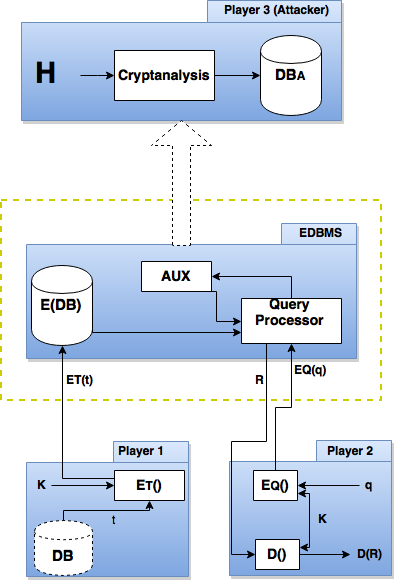
\includegraphics[scale=0.5]{SCONEDB}
     \caption{Figure 1: SCONEDB Model}
\end{figure}
Figure 1 shows SCONEDB model for encrypted database computation. Player 1 is the owner of a database $DB$ on which player 2 can execute certain queries. Instead of processing queries locally Player 1 exports $DB$ to $Encrypted Database Management System$(EDBMS) so Player 2 submits his queries to EDBMS to query DB of Player 1. To secure his data,Player 1 encrypts all tuples in $DB$ before sending them to EDBMS also Player 2 encrypts all his query . In this model EDBMS is considered \textit{trusted but curious}. EDBMS executes an encrypted query on the encrypted database and returns encrypted result $R$($R$ is a set of encrypted tuples which are the answer of a kNN query) to Player 2. To obtain plain result Player 2 applies a decryption function $D$ over $R$.
\\
In this SCONEDB model Player 1 and Player 2 have to agree on common $encryption scheme$. Also Player 1 and Player 2 can be the same actor. In SCONEDB an encryption scheme consists of the following components:
\begin{itemize}
\item \textit{Secret key K}. Encryption and decryption processes requires a key $K$. In this model key is kept private to Player 1 and Player 2.
\item \textit{Database encryption function $E_{T}()$}. The encrypted database $E(DB)$ is obtained by encrypting each tuple $t$ in $DB$ by $E_{T}(t,K)$.
\item \textit{Query encryption function $E_{Q}()$}. Each query $q$ is encrypted by $E_{Q}(q,K)$ before it is submitted to EDBMS
\item \textit{Result decryption function D()} .Each tuple $\hat{t}$ in the encrypted result $R$ is decrypted by $D(\hat{t},K)$
\item \textit{A set of auxiliary operators Aux}. An auxiliary operator
$A_e$ in $Aux$ operates on the encrypted database to obtain information for the purpose of answering queries. In our case $A_e$ returns Euclidean distance between an encrypted tuple $p$ and an encrypted query tuple $q$
\end{itemize}
The main goal in the SCONEDB model is to design an encryption scheme in which $Aux$ can operate on $E(DB)$ to support query processing.
\subsection{Attack models in encrypted databases}
When using SCONEDB model in designing our application we assume that the EDBMS is located at a third party . Therefore we assume that attacker (player 3) sees and controls the environment of EDBMS so attacker has accesses to the encrypted database ,encrypted queries and the ecnrypted results. Also we assume that attacker knows all the components of the scheme except the key. These include
the encryption and decryption procedures ($E_{T}(),E_{Q}()$ and $D()$) also the set of auxiliary operators $Aux$.Attacker's objectives is to recover a plain database $DB_A \subseteq DB$.We assume the attacker is capable to execute PTIME cryptanalysis algorithms with respect to the size of the encrypted database. Main objective is to deny the attacker from obtaining $DB_A$. To better evaluate the strength of an encryption scheme, we classify attackers into different levels based on the knowledge $H$ they possess.
\begin{itemize}
	\item Level 1:\textit{ the attacker observes only encrypted database $E(DB)$, i.e. $H=\langle E(DB) \rangle$. This corresponds to ciphertext-only attack (COA) in cryptography. In practice, there are applications accessed by secluded users, for which other can hardly observe any information other than encrypted data.}
	\item Level 2:\textit{ Apart from $E(DB)$, the attacker knows a set of plain tuples  $P$ in $DB$, but doesn't know their corresponding encrypted values in $E(DB)$, i.e. $H=\langle E(DB), P \rangle$. This corresponds to known-sample attacks in databases in literature. For example, if an attacker observes the encrypted database of a bank and some of his sources are his customers of the bank, he then knows the values of several tuples in the plain database.}
	\item Level 3:\textit{ Apart from $E(DB)$, the attacker knows a set of plain tuples  $P$ in $DB$ and he knows the corresponding encrypted values of those tuples, i.e. $H=\langle E(DB), P, I\rangle$, where $P \subset DB$ and $I(t)=E_T(t, K)$ for all $t \in P$. This corresponds to known known-plaintext attack in cryptography $(KPA)$ or known input-output attack in database literature. For example, if the attacker opens a new account in a bank, and observes only one new encrypted tuple afterwards, he can associate the new account's information (unencrypted) with the encrypted value of the new tuple.}
\end{itemize}
If an encryption scheme resists a higher level attack,it resists a lower level one as well.Level-2 attacks capture practical scenarios this is because in some applications, it is not difficult to observe a small number of plain database tuples. Note that level-3 attacks are rare in practice, since it is not
easy for someone who does not hold the encryption key to associate known plain tuples to their encrypted values.

\subsection{Distance recoverable encryption}
In kNN computation, distances between database points to a query point are computed for finding the nearer neighbors to the query point. To solve the secure kNN problem, it is natural to consider adopting an encryption scheme that allows
the system to compute $d(p_1,p_2)$ on $E(DB)$ for database points $p_1$ and $p_2$ in $DB$. Authors start with the definition of \textit{distance recoverability}.
\\
\\
DEFINITION 1 \textit{(Distance-recoverable encryption DRE)
Given an encryption function E and a key K, let E(p,K) be the encrypted value of a point p in DB. E is distance-recoverable if and only if there exists a computational procedure f such that $\forall p_{1},p_{2}, K, f(E(p_{1},K),E(p_{2},K))=d(p_{1},p_{2})$}.
\newline
\newline
Wong shows that DRE and hence DPT is not secure under level-2 or level3 attacks and introduces a theorem:
\\
\\
THEOREM 1 \textit{Assume a DRE E is used to encrypt DB to get E(DB). A level-3 attacker  with $\langle E(DB), P, I \rangle$ can recover DB if p contains  at least d+1 points $x_{i}$ ($1\le i \le d + 1$) such that the set of vectors $\{x_{j} - x_{i}	| 2 \le j \le d + 1\}$ are linearly independent.} 
\\
\\
\textit{PROOF}  Since the encryption is a DRE, the distance between any two points p and q, d(p, q), can be computed by the attacker using \textit{f(E(p, K), E(q, K))}.Suppose the attacker wants to find the original value of an encrypted point $y' \in E(DB)$. Let the set of known points in $P$ be $\{x_{1},x_{2},...,x_{d'+1}\}$ and $y$ be the original value of $y'$ before encryption . Attacker can set up $d+1$ equations : $d(x_{i},y) = f(I(x_i),y')$ for $i = \overline{1,d+1}$.Each equation thus represents a $d$-dimensional hypersphere. The solution of $y$ lies on the intersection of the hyperspheres.Since $y$ exists in the database, a solution must exist.Author show that if the set of vectors $\{x_j - x_1 \| 2\leq j\leq d_1\}$ are linearly independent, the $d+1$ hypersheres intersect at exactly one point so, $y$ can be uniquely determined. Hence the attacker can recover the entire database $ \square$
\\
\\
The level-3 attack shown above is independent of the implementation of DRE. So, no DRE (e.g. DPT) can survive this level-3 attack.
\subsection{ASYMMETRIC SCALAR-PRODUCT-PRESERVING ENCRYPTION}
The weakness of DRE comes from the fact that the attacker is able to recover
distance information from the encrypted database. More specifically, given any two points $p_1$ and $p_2$ in DB, their distance $d(p_1,p_2)$ can be determined from their encrypted values $E_T(p_1,K)$ and $E_T(p_2,K)$. In kNN search exact distance computation is not necessary we only need a distance comparation. Given two points $p_1$ and $p_2$ in $DB$ we must decide which of the two points is nearer to a query point q. Note that,
\begin{equation}
\begin{aligned}
d(p_1,q) &\geq d(p_1,q)\\
\sqrt{\left \| p_1 \right \|^2 - 2p_1\cdot q + \left \|q \right \|^2} &\geq \sqrt{\left \| p_2 \right \|^2 - 2p_2\cdot q + \left \|q \right \|^2} \\
\left \| p_1 \right \|^2 - \left \| p_2 \right \|^2 + 2(p_2 - p_1)\cdot q &\geq 0
\end{aligned}
\end{equation}
where $\left \| p \right \|$ represents the Euclidean norm of $p$ and $\cdot$ represents scalar product. $\left \| p \right \|^2$ cab be represented by $p\cdot p$. So, the inequality is decomposed to a number of scalar product computations. This suggests a scalar-product-preserving encryption $E_{spp}$ i.e. $\forall p_1, p_2 \in DB,p_1 \cdot p_2 = E_{spp}(p_1,K)\cdot E_{spp}(p_2,K)$,for kNN computation.
\\
\\
\\
THEOREM 2:\textit{Scalar-product-preserving encryption is distance recoverable.}
\\
\\
PROOF. Let $p'_1$ (resp $p'_2$) be the encrypted point of $p_1$(resp $p_2$) in $DB$. Define function $f$ by : \\
\begin{equation}
f(p'_1,p'_2)= \sqrt{p'_1\cdot p'_2 -2(p'_1\cdot p'_2) + p'_2\cdot p'_2}
\end{equation}
Since the encryption preserves scalar product ,we have RHS $=\sqrt{p_1\cdot p_2 -2(p_1\cdot p_2) + p_2\cdot p_2} = d(p_1,p_2)\square$
\\
Wong et al. define several scalar products:
\begin{itemize}
\item (type-1) scalar product of a database point with itself (e.g. $\left\|p\right\|^2$)
\item (type-2) scalar product of a database point with query point
\item (type-3) scalar product of two different database points $p_1$ and $p_2$
\end{itemize}
For our purpose we need an encryption that preserves type-2 but not type-1 or type-3 scalar products. With the precomputed type-1 scalar products, we can verify the inequality of Eq. 1 on the encrypted database to implement the distance comparison operation. Since the encryption does not preserve type-1 or type-3 products, it is not distance recoverable by design. The encryption is thus resilient to level-2 attacks.

DEFINITION 2: \textit{(Asymmetric scalar-product-preserving encryption (ASPE))}\\
\textit{Let E be an encryption function and E(p, K) be the encrypted value of a point p given a key K. E is an ASPE if and only if E preserves type-2 scalar products but not the other two types, i.e.}
\\
\textit{
\begin{enumerate}[(i)]
\item $p_i\cdot q = E(p_i,K)\cdot E(q,K)$ for any $p_i$ in DB and any query point q
\item $p_i\cdot p_j \neq E(p_i,K)\cdot E(p_j,K)$ for any $p_i$ and $p_j$ in DB.
\end{enumerate}}
In Definition 2, we require that the encrypted value of a query $q$ not equal to that of any point $p_j$ in $DB$,even when $q=p_j$.This suggests that query points and database points
should be encrypted differently.That is the encryption functions $E_T()$ and $E_Q()$ in the encryption scheme should be different.

The scalar product of $p$ and $q$ (represented by column vectors) can be represented as $p^{T}Iq$,where $p^T$ is the transpose of $p$ and $I$ is a $d \times d$ identity matrix. $I$ can be decomposed to $MM^{-1}$ for any invertible matrix $M$,i.e., $p^{T}q=(p^{T}M)(M^{-1}q)$. If we set $p' = E_T(p,K) = M^Tp$ (resp. $q' = E_q(q,K) = M^{-1}q$)  it is not possible for one to determine the value of $p$ (resp. $q$) from $p'$ (resp. $q'$) without knowing $M$. Also ,$p'^{T}q' = p^{T}MM^{-1}q = p^{T}q$ i.e , type-2 scalar product is preserved. Suppose $p'_1$ and $p'_2$ are the encrypted points of $p_1$ and $p_2$ in $DB$ respectively ,then $p'^{T}_{1}p'_{2} = p^{T}_{1}MM^{T}p_2$ which is not equal to $p_{1}^{T}p_2$ in general. Type-1 and type-3 scalar products therefore not preserved.So, we ASPE can be implemented by using $M$ and $M^{-1}$ as the transformations for database points and queries .



\subsection{A Secure Scheme Against Level-2 Attacks}
Wong idea is to treat a pre-computed type-1 scalar product $\left\|p\right\|^2$ as the $(d+1)$-st dimension of the point $p$. Given a( $d$-dimensional)  database point $p$ we create a $(d+1)$-dimensional point $\hat{p}$. The first $d$ dimensions of $\hat{p}$ are those of $p$, and the $(d+1)$-st dimension of $\hat{p}$ is set to $-0.5\left\|p\right\|^2$.The extended database points are then transformed(encrypted) using ASPE.

Similarly, we need to extend a query $q$ to a $d+1$-dimensional point $\hat{q}$ before applying ASPE. The simplest way is to set the $(d+1)$-st dimension of $\hat{q}$ to 1. The problem with this method is that the unencrypted query points $\hat{q}$'s all lie on a $d$-dimensional hyperplane with the unit vector in the $(d+1)$-st dimension being the normal of the hyperplane.The attacker can determine the normal of that hyperplane in the transformed space. By considering the normal in the original space and the normal in the transformed space, the attacker obtains some level-3-like information, which is undesirable.

To avoid this problem Wong introduces a random factor. For each query q is generated a random number $r >0$ and scale $\hat{q}$ by $r$, i.e.,$\hat{q} = r(q^T,1)^T$. In THEOREM 3 is shown that this scaling does not affect the correctness of the distance comparison operation
\begin{itemize}
\item \textbf{Key:} a $(d+1)\times (d+1)$ invertible matrix $M$.
\item \textbf{Tuple encryption function $E_T$ :} Consider a database point p
\begin{enumerate}
\item Create a $(d+1)-$dimensional point $\hat{p}$ = $(p^T,-0.5\left \| p \right \|^{2})^T$
\item The encrypted point $p' = M^T\hat{p}.$
\end{enumerate}
\item{\textbf{Query encryption function} $E_Q$}: Consider a query point q
\begin{enumerate}
\item Generate a random number $r > 0$
\item Create a $(d+1)$-dimensional point $\hat{q} = r(q^T,1)^T$
\item The encrypted query point $q' = M^{-1}\hat{q}$
\end{enumerate}
\item \textbf{Distance comparison operator} $A_e$: Let $p'_1$ and $p'_2$ be the encrypted points of $p_1$ and $p_2$ respectively. To determine whether $p_1$ is nearer to a query point $q$ than $p_2$ is, the system checks whether $(p'_1 - p'_2)\cdot q' > 0$,where $q'$ is the encrypted point of $q$.
\item \textbf{Decryption function} $D$: Consider an encrypted point $p'$. The original point $p=\pi_{d}M^{T^{-1}}p'$ where $\pi_d$ is a $d\times (d+1)$ matrix which projects on the first $d$ dimensions and $\pi_d = (I_d,0)$ where $I_d$ is the $d\times d$ identity matrix.
\end{itemize}
THEOREM 3. \textit{Suppose $p'_1$,$p'_2$ and $q'$ are the are the encrypted
points of the database points $p_1$,$p_2$ and the query point q, respectively, scheme correctly determines whether $p_1$ is closer to q than $p_2$ is by evaluating $(p'_1 - p'_2)\cdot q' > 0.$ }
\\
\\
\textit{PROOF:} Note that\\ 
\begin{center}
$(p'_1 - p'_2)\cdot q'$  =  $(p'_1 - p'_2)^T\cdot q'$  =  $(M^T \hat{p_1} -M^T \hat{p_2} )M^{-1}\hat{q}$  =  $(\hat{p_1}-\hat{p_2})^T\hat{q}$
\end{center}
The scalar product of these two $(d+1)$-dimensional points can be represented as:\\
\begin{center}
$(p_1 - p_2)^T(rq)+(-0.5 \left\| p_1\right\|^2 + 0.5\left\| p_2\right\|^2)r = 0.5r(\left\|p_2\right\|^2 -  \left\| p_1\right\|^2 +2(p_1-p_2)^{T}q) = 0.5r(d(p_2,q)-d(p_1,q))$
\end{center}
So, the condition is equivalent to:
\begin{center}
$0.5r(d(p_2,q)-d(p_1,q))>0 \Leftrightarrow (d(p_2,q)>d(p_1,q)\square$
\end{center}
\subsection{Random Asymmetric Splitting}
A level-3 attacker can compute matrix $M$ used in Scheme-1 by setting up enough number of equations using points in $P$ to solve for the unknowns in transformation. In order to make scheme harder to crack Wong et al proposed a method to introduce randomness into the scheme by splitting database point p at each dimension randomly.More specifically, we randomly generate two $d$-dimensional points $p_a$ and $p_b$ (called two $random$ $shares$)
such that for each dimension $i$, we have $p[i] = p_a[i] + p_b[i]$.For simplicity, we write $p = p_a + p_b$. Similarly query point $q$ is splitted. Query and database points can be splitted on each dimension using a split configuration. 
\begin{itemize}
	\item \textbf{Key} two $d' \times d'$ invertible matrices $M_1, M_2$; A bit string S of $d'$ bits: $S_i$ denotes  the $i$-th bit in $S$; $d'-(d+1)$ random numbers $w_{d+2}, w_{d+3},...,w_{d'}$. 
	\item \textbf{Tuple encryption function} $E_T$:	Let $p$ be a database point. 
	\begin{enumerate}
	\item Create a $d'$-dimensional point, where the first $d$ dimensions are copied from $p$. $\hat{p}[d+1]$ is set to $-0.5||p||^2$. For $i=d+2$ to $d'$, if $S_i=1$, we set $\hat{p}[i]$ to $w_i$; otherwise we set $\hat{p}[i]$ to a random number. For the last dimension with which $S_i=0, \hat{p}[i]$ is given a value so that the scalar product over the artificial attributes is 0, or formally $\frac{\sum_{i=d+1}^{s-1}w_it_i}{w_s}$. 
	\item Also we create two shares of $\hat{p}: \hat{p_a}$ and $\hat{p_b}$. For $i=1$ to $d'$, if $S_i=1$ we randomly split the value of $\hat{p}[i]$ into $\hat{p_a}[i]$ and $\hat{p_b}[i]$. If $S_i=0$, both $\hat{p_a}[i]$ and $\hat{p_b}[i]$ are set to $\hat{p}[i]$. 
	\item The encrypted value of $p$ is pair $(p'_a=M_1^T\hat{p}_a,p'_b=M_2^T\hat{p}_b)$. 
	\end{enumerate}
	\item \textbf{Query encryption function} $Q_T$: Let $q$ be a query point. 
	\begin{enumerate}
	\item We generate a random number $r>0$. Also we create a $(d')$-dimensional where the first $d$ dimensions are given by $rq$. The $d+1$-st dimension is set to $r$. For $i=d+2$ to $d'$, if $S_i=0$, we set $\hat{q}[i]$ to $w_i$; otherwise we set $\hat{q}[i]$ to a random number. For the last dimension with which $S_i=1, \hat{q}[i]$ is given a value so that the scalar product over the artificial attributes is 0, or formally $\frac{\sum_{i=d+1}^{s-1}w_it_i}{w_s}$.
	\item Also we create two shares of $\hat{q}: \hat{q_a}$ and $\hat{q_b}$. For $i=1$ to $d'$, if $S_i=0$ we randomly split the value of $\hat{q}[i]$ into $\hat{q_a}[i]$ and $\hat{q_b}[i]$. If $S_i=1$, both $\hat{q_a}[i]$ and $\hat{q_b}[i]$ are set to $\hat{q}[i]$.
	\item The encrypted value of $q$ is pair $(q'_a=M_1^{-1}\hat{q}_a,q'_b=M_2^{-1}\hat{q}_b)$.
	\end{enumerate}
	\item \textbf{Distance comparison function} $A_e$: Let $(p'_{1a},p'_{1b})$ and $(p'_{2a},p'_{2b})$ be encrypted values for database points $p_1$ and $p_2$ and $(q'_a, q'_b)$ encrypted value for query point $q$. The system will check whether $(p'_{1a} - p'_{2a}) \cdot q'_a + (p'_{1b} - p'_{2b}) > 0$. If this condition is true then $p_1$ is closer to $q$ than $p_2$. 
	\item \textbf{Decryption function} $D$: Let $(p'_a, p'_b)$ be an encrypted point. First, we recover two shares and extract the first d dimensions in it: $p_a=\pi_{d}M_1^{T^{-1}}p'_a$ and $p_b=\pi_{d}M_2^{T^{-1}}p'_b$ where $\pi_d$ is $d \times (d+1)$ dimensional matrix which projects on first $d$ dimensions. Then, $p[i]$ is equal to $p_a[i]$ if $S_i=0$; or $p_a[i]+p_b[i]$ if $S_i=1$.
\end{itemize}

Relative to this scheme next theorem is essential. 
\\
\\
THEOREM 6 \textit{Random Asymmetric Splitting is resilient against level 3 attacks if the attacker cannot derive the splitting configuration, i.e., the bit string S of the key in previous scheme.}
\\
\\
\textit{PROOF:} If we consider the knowledge of tha attacker to be $H=\langle E(DB), P, I\rangle$, without loss of generality, we assume $d'=d+1$, i.e., no artificial attributes are added. (The addition of artificial attributes will only increase the security of scheme). From definition of level 3 attacks, for any point $p_i \in P$, attacker knows encrypted values $(p'_{ia}, p'_{ib})$. If the attacker does not know the splitting configuration, he has to model $\hat{p_ia}$ and $\hat{p_ib}$ as two random $d'$-dimensional vectors. The equations for solving the transformation matrices are: $M_1^T\hat{p_a}=p'_a$ and $M_2^T\hat{p_b}=p'_b$, where $M_1$ and $M_2$ are two $d' \times d'$ unknown matrices. There are $2d'|P|$ unknowns in $\hat{p_{ia}}$ and $2d'^2$ unknowns in $M_1$ and $M_2$. Since there are only $2d'|P|$ equations, which are less than number of unknowns, the attacker does not have sufficient information to solve for the transformation matrices. Hence, second Wong scheme is resilient against this level-3 attack. $\square$ 


\section{Our contribution on fixing KPA attack on ASPE}
\subsection{Fixed protocol}
In this section we present our fix for Chunsheng attack on ASPE.

\begin{itemize}
	\item{\textbf{Key}}
	Given parameters $\lambda$,$\beta$ the dimensions $d(\lambda)$,$d'(\lambda)$ of a database point $p$, and encrypted value of $p$:
	
	\begin{enumerate}
		\item Choose two invertible matrices $M_{1},M_{2}\in Q^{d' \times d'}$ , such that $\left |M_{k}\left [ i,j \right ]  \right | \leq 2^{\lambda} , k \in \left \langle2 \right \rangle i,j \in \left \langle d' \right \rangle $
		
		\item Randomly generate bit string $s$,$\in \left \{ 0,1\right \}^{d'-(d+1)}$ 
		\item Choose $d' - \left ( d+1 \right )$ random numbers $w_{d+2},w_{d+3}, \ldots ,w_{d'} \in Q$ such that $w_{j} \ne 0$ and $\left | w_{j} \right | \leq 2^{\lambda},j \in \left \langle d' \right \rangle \setminus  \left \langle d+1 \right \rangle$
		
		\item Choose a permutation matrix $P_{\pi},P_{\pi} \in \left\{0,1\right\}^{d' \times d'}$ 
		such that $\nexists P_{\pi}\left[i,i\right] = 1, \nexists P_{\pi}\left[i,j\right] =P_{\pi}\left[i,k\right] = 1, j\neq k$ and $\nexists P_{\pi}\left[i,j\right] =P_{\pi}\left[k,j\right] = 1, i\neq k ;i,j,k\in \left \langle d'\right \rangle$
		\item Output secret key $sk = \left \{ M_{1} ,M_{2} ,s ,\left \{ w_{j},j \in \left \langle d' \right \rangle \setminus \left \langle d+1 \right \rangle \right \},P_{\pi} \right  \}$
	\end{enumerate}
	
	\item{\textbf{Encryption algorithm}}
	Given a $d$-dimensional database point $p$ and secret key $sk$:
	\begin{enumerate}
		\item Create a $d'$-dimensional $\tilde p$:
		\begin{itemize}
			\item $\tilde{p}[i] = p[i],\forall i \in \left \langle d \right \rangle$
			\item $\tilde{p}[d+1] = -0.5\left \|  p\right \|^{2}$
			\item
			$\left\{\begin{matrix}
			\tilde{p}[i] = w_i,if\;s[i] = 1 & &\\ 
			& & ,i\in \left \langle d' \right \rangle \setminus  \left \langle d+1 \right \rangle \\
			\tilde{p}[i] = r_i,if\;s[i] = 0 & &
			\end{matrix}\right.$
			\\
			\\
			where $r_i\in Q$ and $\left|r_i\right|\leq 2^\lambda$;
			\item
			Let k = $max\left \{ j\mid s\left [ j \right ] = 0,j\in\left \langle d' \right \rangle\setminus \left \langle d+1 \right \rangle \right \}$
			\\
			\\
			$    \tilde{p}\left [ k \right ] = -\left ( \sum\limits_{s_j=0,j\geq d+2,j\neq k}^{}\tilde{p}\left [ j \right ]w_j\right)/w_k$
		\end{itemize}
		\item
		Permute $\tilde{p}$ using $P_\pi$:
		\begin{itemize}
			\item 
			$\hat{p} =\tilde{p}^{T}P_\pi $
		\end{itemize}
		\item
		Split $\hat{p}$ into $\hat{p}_a$ and $\hat{p}_b$ using $s$:
		\begin{itemize}
			\item Randomly choose $R \in Q^{n}$,such that $0<\left | R\left [ i \right ]  \right | \leq 2^\lambda ,i \in \left \langle d' \right \rangle$ 
			
			\item 
			$\left\{\begin{matrix}
			\hat{p_a}\left [ i \right ] = \hat{p}\left [ i \right ] + R\left [ i \right ],& \hat{p_b}\left [ i \right ] = \hat{p}\left [ i \right ] - R\left [ i \right ],&if\,\,s\left [ i \right ]=1 &\\ 
			& & &,i\in \left \langle d' \right \rangle  \\
			\hat{p_a}\left [ i \right ] = \hat{p}\left [ i \right ] - R\left [ i \right ],&
			\hat{p_b}\left [ i \right ] = \hat{p}\left [ i \right ] + R\left [ i \right ],&if\,\,s\left [ i \right ]=0 &
			\end{matrix}\right.$
		\end{itemize}
		\item
		Generate encrypted value of $p$:
		\begin{itemize}
			\item $\overline{p}=\left ( \overline{p}_{a} = M^{T}_{1}\hat{p}_{a},\overline{p}_{b} = M^{T}_{2}\hat{p}_{b}\right )$
		\end{itemize}
	\end{enumerate}
	
	\item{\textbf{Query encryption algorithm}}
	Given a $d$-dimensional query point $q$ and secret key $sk$:
	\begin{enumerate}
		\item Create a $d'$-dimensional $\tilde q$:
		\begin{itemize}
			\item Choose randomly $r\in Q$ with $0<r\leq 2^\lambda$
			\item $\tilde{q}[i] = rq[i],\forall i \in \left \langle d \right \rangle$
			\item $\tilde{q}[d+1] = r$
			\item
			$\left\{\begin{matrix}
			\tilde{p}[i] = w_i,if\;s[i] = 0 & &\\ 
			& & ,i\in \left \langle d' \right \rangle \setminus  \left \langle d+1 \right \rangle \\
			\tilde{p}[i] = r_i,if\;s[i] = 1 & &
			\end{matrix}\right.$
			\\
			\\
			where $r_i\in Q$ and $\left|r_i\right|\leq 2^\lambda$;
			\item
			Let k = $max\left \{ j\mid s\left [ j \right ] = 1,j\in\left \langle d' \right \rangle\setminus \left \langle d+1 \right \rangle \right \}$
			\\
			\\
			$    \tilde{q}\left [ k \right ] = -\left ( \sum\limits_{s_j=0,j\geq d+2,j\neq k}^{}r_{j}w_j\right)/w_k$
		\end{itemize}
		\item
		Permute $\tilde{q}$ using $P_\pi$:
		\begin{itemize}
			\item 
			$\hat{q} =\tilde{q}^{T}P_\pi $
		\end{itemize}
		\item
		Split $\hat{q}$ into $\hat{q}_a$ and $\hat{q}_b$ using $sw$:
		\begin{itemize}
			\item 
			
			$\hat{q_a}\left [ i \right ] = \hat{q}\left [ i \right ],\hat{q_b}\left [ i \right ] = \hat{q}\left [ i \right ] ,i\in \left \langle d' \right \rangle  \\
			.$
		\end{itemize}
		\item
		Generate encrypted value of $q$:
		\begin{itemize}
			\item $\overline{q}=\left ( \overline{q}_{a} = M^{-1}_{1}\hat{q}_{a},\overline{q}_{b} = M^{-1}_{2}\hat{q}_{b}\right )$
		\end{itemize}
	\end{enumerate}
	\item{\textbf{Decryption algorithm }}: $D$ Let $(p'_a, p'_b)$ be an encrypted point. First, we recover two shares and extract the first d dimensions in it: $p_a=\pi_{d}M_{1}^{T^{-1}}p'_a$ and $p_b=\pi_{d}M_{2}^{T^{-1}}p'_b$ where $\pi_d$ is $d \times (d+1)$ dimensional matrix which projects on first $d$ dimensions. Then, $2p[i]$ is equal to $(p_a[i]+p_b[i])$. 
	\item{\textbf{Distance comparison algorithm}}
	Given the encrypted value $\overline{p}^{j} = \left ( \overline{p}^{j}_{a}, \overline{p}^{j}_{b}\right ),\overline{q}^{j} = \left ( \overline{q}_{a}, \overline{q}_{b}\right )$ of two database points $p_j,j\in \left \langle 2 \right \rangle$,a query point $q$:
	\begin{itemize}
		\item if $\left ( \overline{p}_{a}^{1} - \overline{p}_{a}^{2} \right )\overline{q}_{a}
		+ \left ( \overline{p}_{b}^{1} - \overline{p}_{b}^{2} \right )\overline{q}_{b} > 0$ then $p_1$ is nearer to $q$;otherwise $p_2$ is nearer to $q$.
	\end{itemize}
\end{itemize}
\subsection{Correctness proof}
Now we will discuss correctness of our algorithm. There are several aspects that we should present related to second Wong protocol. First of all we should make more clear what exactly make it vulnerable. The answer at this question is exposed in theorem 6. \\
So, what is the problem with Wongs' protocol. Answer is simple, it allows an attacker to make distinction between cases when bit values of split configuration string $s$ are used. So in our opinion, the phase that implies split of extended point can be done somehow different. This we showed in our fix. Also this fix implies change of query encryption algorithm. Now we will present our proof for search correctness using scheme above. After we made this proof, we observed that there can be done several changes in order to improve security. We will discuss these improvements later.
\\
\\
\textit{PROOF:} Let $(p'^1_a, p'^1_b)$ be the encrypted value for database point $p^1$, $(p'^2_a, p'^2_b)$ be the encrypted value for database point $p^2$ and $(q'_a, q'_b)$ be the encrypted value for a query point $q$.

Now, given splitting configuration string, given value on index $i, s[i], i \in \langle d\rangle$, our equation has following behavior:

If we will not respect this simple steps, asymmetric scalar product encryption will work, but will not have proper distance comparison properties, which is essential in our scenario. However, we showed that our changes to Wong protocol are not changing its behavior and represent a fix for Chunsheng attack because changes that are made at splitting step in encryption phase are similar from the attacker point of view. This mean that he shouldn't be able to recover splitting configuration string and should not be able to use it in his way of recovering secret key, and of course to recover plain database data.
\section{Practical implementation}
In this section I present how we can use ASPE in securing databases and queries over them. To implement ASPEDB I use .Net framework and C\# as programming language. To store data I use MongoDB noSql database.
\subsection{ASPE DataBase}
Now a detailed application 

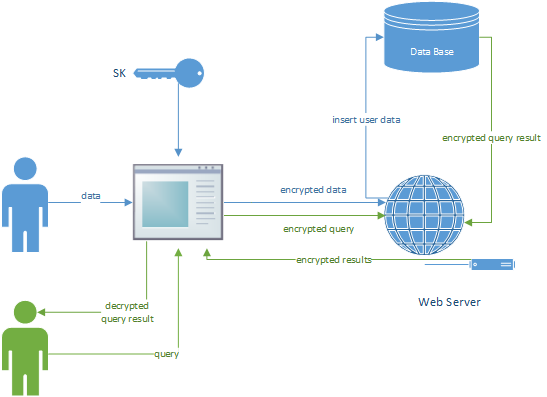
\includegraphics{application}
\subsection{Data type conversion}
\subsection{CRUD Operation}
\subsubsection{Create}
\subsubsection{Read}
\subsubsection{Update}
\subsubsection{Delete}
\subsection{Benchmarks}

\section{Conclusion}



\bigskip{}



\pagebreak{}


\begin{thebibliography}{4}
	\bibitem{Wong}
	W. K. Wong, David W. Cheung, Ben Kao, Nikos Mamoulis, Secure kNN Computation on Encrypted Databases, 2009, Proceedings of the 2009 ACM SIGMOD International Conference on Management of data,
	Pages 139-152;
	\bibitem{Chunsheng} Gu Chunsheng, Gu Jixing, Known-plaintext attack on secure kNN computation on
	encrypted databases, 2014, Security and communication networks;
	\bibitem{Choi} Sunoh Choi, Gabriel Ghinita, Elisa Bertino, A Privacy-Enhancing Content-Based Publish/Subscribe System Using Scalar Product Preserving, 2010, DEXA'10 Proceedings of the 21st international conference on Database and expert systems applications: Part I,
	Pages 368-384; 

\end{thebibliography}
\end{document}
